\chapter{Validation Loss Across Transformer Sizes}
\label{app:heads_val_loss}

All four runs converge to essentially the same floor, with best values of
$0.0329$--$0.0332$. Larger models descend faster per epoch but reach only slightly 
lower asymptote, while the lightweight 1h1d configuration matches them given
enough epochs.

The training budgets were not equal. All runs were limited to 24\,h
on DelftBlue, and only the 1h1d configuration completed the full 400 epochs (in
14\,h); the 2h2d, 4h3d and 8h6d runs timed out at progressively fewer epochs
(360, 266, 140 respectively) because each epoch is more expensive
for the larger models. That the larger variants matched 1h1d \emph{despite}
receiving less training reinforces the conclusion that the fusion module
saturates at minimal capacity, and that the preferred 1h1d configuration
sacrifices no reconstruction accuracy.

\begin{figure}[htbp]
  \centering
  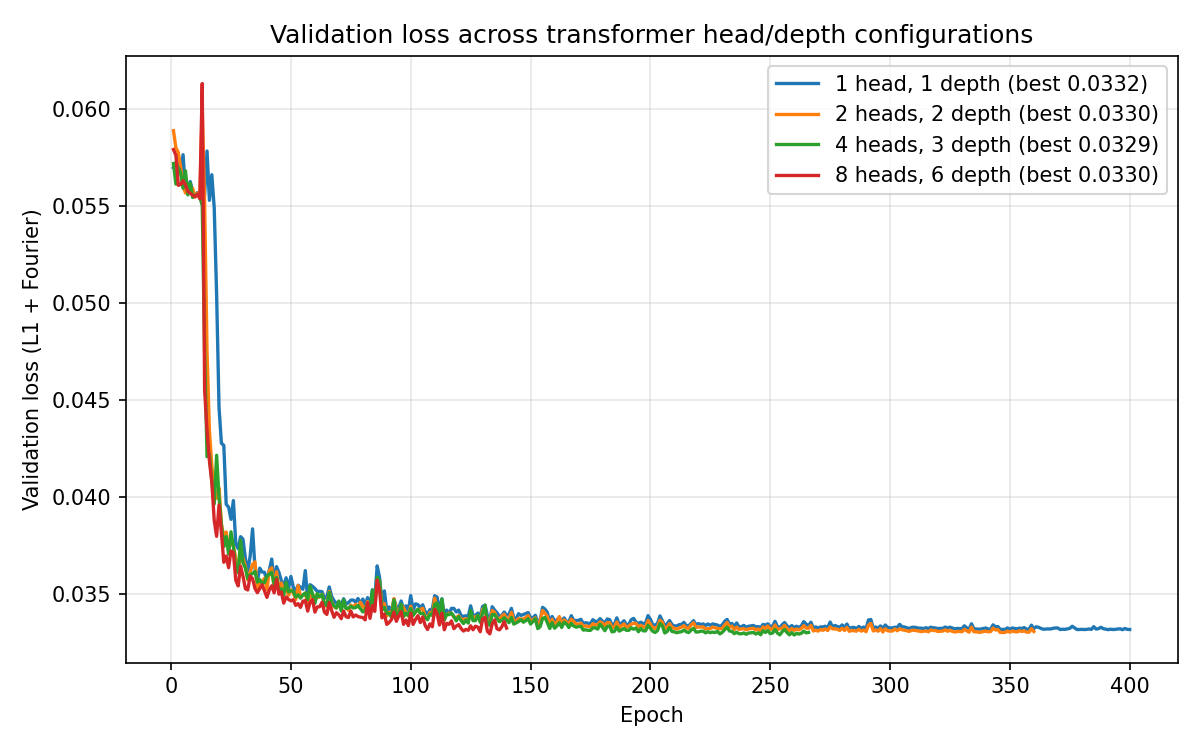
\includegraphics[width=\linewidth]{figures/heads_val_loss.png}
  \caption{Validation loss (L1 + Fourier) per epoch during training for the four
  Transformer head/depth configurations. All converge to nearly identical loss.
  Runs were limited to 24\,h, so the larger variants completed
  fewer epochs than 1h1d.}
  \label{fig:heads_val_loss}
\end{figure}
